\normalfalse \difficiletrue \tdifficilefalse
\correctionfalse

%\UPSTIidClasse{11} % 11 sup, 12 spé
%\newcommand{\UPSTIidClasse}{12}

\exer{Barrière Sympact avec galet $\star\star$ \label{C2:06:15}}
\setcounter{question}{0}\UPSTIcompetence[2]{B2-13}\UPSTIcompetence[2]{C2-05}\UPSTIcompetence[2]{C2-06}
\index{Compétence C2-05}
\index{Compétence C2-06}
\index{Compétence B2-13}
\index{Barrière Sympact}
\index{Croix de Malte}
\ifcorrection
\else
\marginnote{\textbf{Pas de corrigé pour cet exercice.}}
\fi

\ifprof
\else

Soit le mécanisme suivant. On a $\vect{AC}=H\vect{j_0}$ et $\vect{CB}=R\vect{i_1}$. De plus, 
$H=\SI{120}{mm}$ et $R=\SI{40}{mm}$. 

\begin{center}
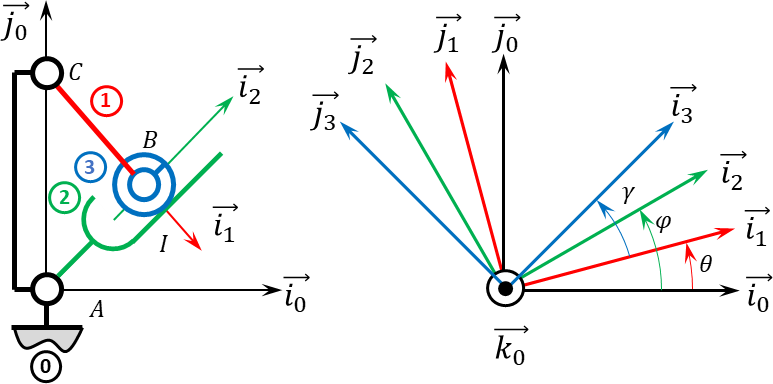
\includegraphics[width=\linewidth]{15_01}
\end{center}
\fi


\question{Tracer le graphe des liaisons.}
\ifprof
\else
\fi

\question{Exprimer $ \varphi(t)$ en fonction de $\theta(t)$.}
\ifprof
\else
\fi

\question{Exprimer $\dot{\varphi}(t)$ en fonction de $\dot{\theta}(t)$.}
\ifprof
\else
\fi

\question{En utilisant la condition de roulement sans glissement au point $I$, déterminer $\gamma(t)$ et $\dot{\gamma}(t)$.}
\ifprof
\else
\fi

\question{En utilisant Python, tracer $\dot{\varphi}(t)$ en fonction de $\dot{\theta}(t)$. On considérera que la fréquence de rotation de la pièce \textbf{1} est de 10 tours par minute.}
\ifprof
\else
\fi


\ifprof
\else
\begin{flushright}
\footnotesize{Corrigé  voir \ref{C2:06:15}.}
\end{flushright}%
\fi